\documentclass[a4paper,12pt]{report}
\usepackage{graphicx} 
\usepackage{geometry}
\usepackage{setspace}
\usepackage{titlesec} 
\titlespacing*{\subsection}{0pt}{4pt}{2pt}
\setlength{\parskip}{2pt}
\usepackage{ragged2e} 
\usepackage{tabularx}
\usepackage{needspace}
\usepackage{enumitem}
\usepackage{graphicx}
\usepackage{float}
\usepackage{subcaption}
\usepackage{tocloft}
\usepackage{listings}
\usepackage{xcolor}

\lstset{
    basicstyle=\ttfamily\small,
    breaklines=true,
    frame=single,
    showstringspaces=false
}
\setlist{noitemsep, topsep=2pt}
\titlespacing*{\subsection}{0pt}{6pt}{4pt}
\raggedbottom
\setlist[enumerate]{itemsep=4pt, topsep=4pt}
\flushbottom
\geometry{margin=1in}
\onehalfspacing
\raggedbottom

\titleformat{\section}
  {\normalfont\huge\bfseries}
  {\thesection}{1em}{}

\begin{document}

% -------------------- TITLE PAGE --------------------
\begin{titlepage}
\centering

{\LARGE \textbf{SkillNet -- Campus Marketplace}}

\vfill

{\Large \textbf{PCCST402 -- DATABASE MANAGEMENT SYSTEMS}}

\vfill

\textbf{Course Project Report}

\vfill

\textbf{Submitted by}

\vspace{5mm}

\textbf{APOORV NAMBIAR (Reg No: MUT24CS043)}\\
\textbf{BALASANKAR C B (Reg No: MUT24CS049)}\\
\textbf{JOEL SANTHOSH (Reg No: MUT24CS087)}\\
\textbf{RICHARD SHAJI MEKKADEN (Reg No: MUT24CS127)}\\
\textbf{VISHNU PRASAD PV (Reg No: MUT24CS150)}

\vfill

% Placeholder for the logo image
\includegraphics[width=0.75\textwidth]{Mits_New.jpeg}

\vfill

\textbf{DEPARTMENT OF COMPUTER SCIENCE AND ENGINEERING}\\
(Affiliated to APJ Abdul Kalam Technological University)\\
Kochi - 682308

\vfill

\textbf{March 2026}

\end{titlepage}

% -------------------- CERTIFICATE --------------------
\chapter*{CERTIFICATE}
\vspace{3cm}

This is to certify that the Project report entitled \textbf{SkillNet -- Campus Marketplace} submitted by Apoorv Nambiar (MUT24CS043), Balasankar C B (MUT24CS049), Joel Santhosh (MUT24CS087), Richard Shaji Mekkaden (MUT24CS127) and Vishnu Prasad PV (MUT24CS150) of Semester IV is a bonafide account of the work done by them under our supervision during the academic year 2025-26.
This project work has been carried out in the Department of Computer Science and Engineering, Muthoot Institute of Technology and Science, under the guidance of Lithiya Sara Babu, Assistant Professor, and has not been submitted elsewhere for any other
purpose.
\vspace{3cm}

\textbf{\\Lithiya Sara Babu}\\
Faculty-In-Charge
\vspace{3cm}
\\
Place: Kochi\\
Date: 30/03/2026

\newpage

% -------------------- TOC --------------------

\tableofcontents
\newpage

% -------------------- ABSTRACT --------------------
\chapter{ABSTRACT}

This project presents the design and development of a web-based premium peer-to-peer campus marketplace named \textbf{SkillNet}. The system is developed using modern web technologies including React for the frontend interface and Node.js with PostgreSQL for the backend operations. It provides an efficient platform for students to securely buy, sell, and trade items with verified campus peers in an organized manner.

\vspace{0.3cm}

The application offers specialized user experiences by incorporating modern design principles like glassmorphism. Users can seamlessly register, log in, browse through a market feed of available listings, post their unique listings, and proceed to a streamlined checkout. Every transaction ensures that verified students within a contained campus environment can exchange goods effectively.

\vspace{0.3cm}

PostgreSQL is used as the foundational backend database to ensure highly scalable and strictly structured relational data storage. Utilizing Node.js REST APIs for efficient data operations, the system enforces secure and optimized interactions such as fast product fetching, dynamic listing additions, and real-time UI updates. SkillNet successfully replaces unstructured, ad-hoc trading groups (e.g., WhatsApp chats) with a centralized, reliable, and smooth student marketplace.

% -------------------- INTRODUCTION --------------------
\chapter{INTRODUCTION}

\section{Purpose of the System}

The purpose of this project is to conceptualize, design, and develop a comprehensive web-based platform, SkillNet, functioning as a dedicated campus marketplace. It replaces manual and scattered methods of trading among students with a centralized and efficient digital solution. It enables students to easily upload item listings, categorize them, browse actively available items, and finalize secure P2P transactions. The system also introduces strict validations to operate specifically within a campus domain, ensuring safety and demonstrating key database properties using a robust RDBMS.

\section{Relevance and Scope}

Campus trading is an essential activity where students constantly need to exchange items like textbooks, electronics, and hostel accessories. Traditional methods and unmoderated chat groups often lead to trust issues, inefficiencies, duplicate postings, and lost messages. SkillNet provides a structured, responsive, and reliable digital solution customized entirely for campus life.

The scope of the system includes user authentication, posting new item listings with details and images, browsing a lively market feed, viewing active user listings, and simulated checkout processing. The database handles user sessions, product inventory, and services offered by the student community.

% -------------------- SYSTEM ANALYSIS --------------------
\chapter{PROBLEM DEFINITION}

\section{Problem Statement}

Currently, students lack a unified, trustworthy, and visually appealing platform to exchange goods within the campus. They resort to fragmented and disorganized social media group chats. Trading within such unmoderated groups makes it difficult to verify users, update statuses of sold products, search effectively for active listings, and safely arrange the final exchange of goods. It routinely causes data redundancy and clutter.

Therefore, an intuitive marketplace is strictly required that structurally encapsulates database entities, offers refined retrieval mechanisms, authenticates parties, and guarantees the streamlined management of campus commerce.

\section{Objectives}

\begin{itemize}
\item Develop a centralized online marketplace tailored solely for campus students.
\item Implement an effective relational schema using PostgreSQL for data integrity.
\item Craft a premium user interface employing modern Glassmorphic design and smooth web animations.
\item Ensure effective real-time data flow consisting of product registration, searching, and simulated billing.
\item Drastically reduce search time by organizing listings efficiently over an intuitive Market Feed.
\end{itemize}

% -------------------- REQUIREMENTS --------------------
\chapter{REQUIREMENT ANALYSIS}

\section{Software Requirements}
\begin{itemize}
\item JavaScript / Node.js
\item React (Vite framework)
\item Express.js 
\item PostgreSQL (Database engine, via pg)
\item Modern Web Browser (Chrome, Firefox, Safari)
\end{itemize}

\section{Functional Requirements}
\begin{itemize}
\item Secure Student User Login and Registration 
\item Dynamic product listings feed (Market Feed)
\item Detailed product and service submission system
\item Automated campus checkout and digital receipt generation
\end{itemize}

\section{Non-Functional Requirements}
\begin{itemize}
\item High Performance and fast rendering (Optimized React states)
\item Mobile-responsive UI design
\item ACID compliance natively inherited through PostgreSQL
\item Robust error handling and form validation
\item Scalable Database Architecture
\end{itemize}

% -------------------- SYSTEM DESIGN --------------------
\chapter{SYSTEM DESIGN}

\section{Architecture}

The system conforms to a modern PERN architecture (PostgreSQL, Express, React, Node.js). Users interact directly with the highly dynamic frontend React application, styled using CSS with premium glassmorphism layouts. When an operation implies submitting a listing or fetching the latest feed, dynamic HTTP calls are forwarded to the centralized Node.js/Express.js backend server. The backend actively interfaces with the PostgreSQL relational database handling SQL queries, constraints validation, and updates. The architecture seamlessly separates the client UI logic, server-side data routing, and long-term persistence layer to remain maintainable.

\section{Technologies Used}

\subsection{Frontend}
The frontend operates largely on React utilizing Vite for robust compilation and hot-reloading. The styling deliberately leverages sophisticated modern aesthetics using customized CSS (tailored animations, vibrant gradients, and glassmorphic layers). A Single Page Application (SPA) structure ensures that navigating between components happens instantly without reloading the entire application interface. 

\subsection{Backend}
The backend logic operates on a Node.js runtime executing an Express.js server natively designed to manage RESTful endpoints asynchronously. It intercepts network requests (GET, POST), validates the transmitted payload securely, applies any required campus-side business logic, and delegates queries to the database connector. 

\subsection{Database}
PostgreSQL is integrated natively as the robust Relational Database Management System (RDBMS). It facilitates reliable data management utilizing structured schemas, constraints, and relationships. Standard SQL commands easily perform Create, Read, Update, and Delete operations for strict marketplace property maintenance.

\section{Database Design and Concepts}

The fundamental architecture of the system leverages critical Database Management Systems (DBMS) properties natively embedded within PostgreSQL to assure long-term reliability.

\subsection{DBMS Concepts Implemented}

\begin{itemize}
\item \textbf{Entity-Relationship \& Normalization}: The database schemas are structurally partitioned into distinct entities (Users, Products, Services) ensuring adherence to the Third Normal Form (3NF). This design completely eliminates data redundancy and prevents insertion, update, or deletion anomalies.
\item \textbf{Referential Integrity}: Employing \texttt{FOREIGN KEY} constraints strictly binds active listings to valid users. The DBMS automatically prevents the presence of "orphan" products by strictly auditing user references upon any deletion attempt.
\item \textbf{ACID Properties}: By encapsulating operations in atomic transactions, the application ensures Atomicity, Consistency, Isolation, and Durability (ACID), guaranteeing that complex interactions like peer-to-peer exchanges and registrations never end in intermediate states or dirty reads.
\end{itemize}

\subsection{Tables Used}

\begin{itemize}
\item \textbf{users}: Stores core account details utilizing a \texttt{PRIMARY KEY} (\texttt{user\_id}) along with a \texttt{UNIQUE} constraint on the \texttt{email} field to guarantee distinct user access.
\item \textbf{products}: Contains marketplace listings designated as physical items containing attributes like title, price, and descriptive text. It explicitly relies on the \texttt{user\_id} as a \texttt{FOREIGN KEY}. A parameterized \texttt{CHECK} constraint ensures the \texttt{pricing\_model} precisely conforms to designated formats ('PAID', 'FREE', 'CHAI').
\item \textbf{services}: Maintains service-based marketplace listings employing an identical robust column architecture but logically separated to segment queries efficiently for runtime optimization.
\end{itemize}

\subsection{Class Diagram}

The logical structuring mapping out entities, attributes, and cardinality corresponding to our schema design is visually compiled below.

\begin{figure}[H]
\centering
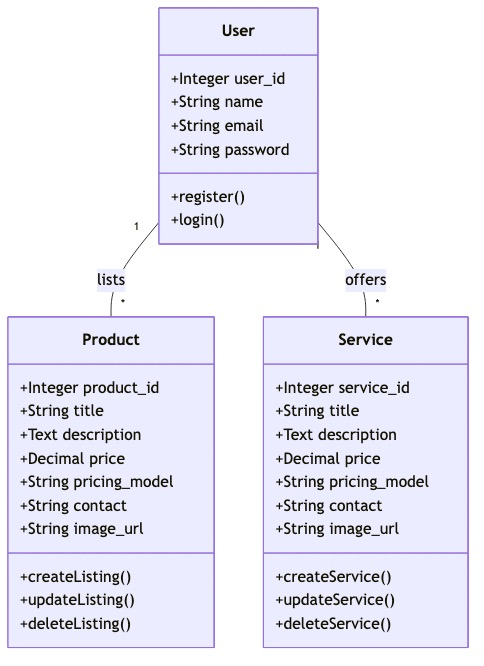
\includegraphics[width=0.8\textwidth]{classdigarm.jpeg}
\caption{System Class Diagram mapping DBMS Entity Relationships}
\end{figure}

% -------------------- IMPLEMENTATION --------------------
\chapter{IMPLEMENTATION}

\section{Frontend Module}

The UI heavily revolves around localized components interacting systematically to formulate a seamless user flow. The \texttt{MarketFeed} seamlessly requests product arrays dynamically and lists them within premium interactive card layouts. User input logic exists deeply within the \texttt{CreateListing} forms supporting rich descriptors before being sent securely to the backend.

\section{Backend \& Database Module}

Node.js isolates connection pools targeting the local or remote PostgreSQL instance securely handling independent API endpoints representing logical marketplace functions. Routes define transaction statements required to safely insert or retrieve structured tabular data avoiding race conditions and anomalies using primary keys.

\newpage

\section{Complete Source Code (Database Excerpt)}

The following code excerpt presents the actual database initialization script located in \texttt{backend/database.js}. This layer leverages the \texttt{pg} dependency constructing critical tables and seeding fundamental schemas connecting the backend correctly to our PostgreSQL instance.

\begin{lstlisting}[language=JavaScript]
//dotenv is a package to use  env file to get key-value pairs
require('dotenv').config();
//pg is a package to connect to postgresql
const pg = require('pg'); //library
//creates the connection pool
const Pool = pg.Pool;

const pool = new Pool({
  connectionString: process.env.DATABASE_URL,
  ssl: { rejectUnauthorized: false }
});

async function initializeDatabase() {
  const createUsersTable = `
    CREATE TABLE IF NOT EXISTS users (
      user_id  SERIAL PRIMARY KEY,
      name     VARCHAR(255),
      email    VARCHAR(255) NOT NULL UNIQUE,
      password VARCHAR(255) NOT NULL
    );
  `;
  const addNameColumnIfMissing = `
    ALTER TABLE users ADD COLUMN IF NOT EXISTS name VARCHAR(255);
  `;
  const createProductsTable = `
    CREATE TABLE IF NOT EXISTS products (
      product_id    SERIAL PRIMARY KEY,
      title         VARCHAR(255) NOT NULL,
      description   TEXT,
      price         DECIMAL(10, 2) NOT NULL DEFAULT 0,
      pricing_model VARCHAR(50) NOT NULL CHECK (pricing_model IN ('PAID', 'FREE', 'CHAI')),
      contact       VARCHAR(255),
      image_url     TEXT,
      user_id       INTEGER NOT NULL REFERENCES users(user_id)
    );
  `;
  const createServicesTable = `
    CREATE TABLE IF NOT EXISTS services (
      service_id    SERIAL PRIMARY KEY,
      title         VARCHAR(255) NOT NULL,
      description   TEXT,
      price         DECIMAL(10, 2) NOT NULL DEFAULT 0,
      pricing_model VARCHAR(50) NOT NULL CHECK (pricing_model IN ('PAID', 'FREE', 'CHAI')),
      contact       VARCHAR(255),
      image_url     TEXT,
      user_id       INTEGER NOT NULL REFERENCES users(user_id)
    );
  `;
  
  // Executing table schemas asynchronously using the pg pool
  console.log('EXECUTING DB COMMAND: ', createUsersTable);
  await pool.query(createUsersTable);
  console.log('EXECUTING DB COMMAND: ', addNameColumnIfMissing);
  await pool.query(addNameColumnIfMissing);
  console.log('EXECUTING DB COMMAND: ', createProductsTable);
  await pool.query(createProductsTable);
  console.log('EXECUTING DB COMMAND: ', createServicesTable);
  await pool.query(createServicesTable);

  console.log('Database initialized successfully.');
}

module.exports = { pool, initializeDatabase };
\end{lstlisting}

% -------------------- RESULTS --------------------
\chapter{RESULTS AND DISCUSSION}

\section{Market Feed Interface}

The Market Feed interface displays active product and service listings dynamically fetched from the database, allowing users to browse items.

\begin{figure}[H]
\centering
\includegraphics[width=0.85\textwidth]{market_feed.jpeg}
\caption{Market Feed Interface}
\end{figure}

\section{Post Listing Interface}

The Post Listing interface enables students to create new listings by entering product details, pricing, and images seamlessly.

\begin{figure}[H]
\centering
\includegraphics[width=0.85\textwidth]{post_listing.jpeg}
\caption{Post Listing Interface}
\end{figure}

\section{Detailed Listing View}

Users can view individual listings in detail, showcasing full item descriptions, pricing models, and contact information.

\begin{figure}[H]
\centering
\includegraphics[width=0.85\textwidth]{listing_detail.jpeg}
\caption{Detailed Listing View}
\end{figure}

\section{Checkout Interface}

The streamlined checkout process provides a modal for users to securely finalize their P2P transactions.

\begin{figure}[H]
\centering
\includegraphics[width=0.85\textwidth]{checkout.jpeg}
\caption{Checkout Interface}
\end{figure}

% -------------------- CONCLUSION --------------------
\chapter{CONCLUSION AND REFERENCES}

\section{Conclusion}

This project presents the comprehensive design and active implementation of the \textbf{SkillNet Campus Marketplace} utilizing the PERN technological stack (PostgreSQL, Express, React, Node.js). 

It fully automates product/service submission, category browsing, and simulated P2P checkout operations thereby drastically minimizing redundancy and scaling issues native to manual campus transactions. The integrated relational database assures that accurate user listings remain consistently structured, leveraging constraints effectively over conventional unstructured designs. The system strictly delivers a modern, robust, and highly responsive web application actively illustrating complex RDBMS management paradigms in real-world environments.

\section{References}

\begin{enumerate}
\item Abraham Silberschatz, Henry F. Korth, and S. Sudarshan, \textit{Database System Concepts}, McGraw-Hill, 7th Edition, 2019.

\item PostgreSQL Global Development Group, \textit{https://www.postgresql.org/docs/}

\item Node.js Foundation, \textit{https://nodejs.org/docs}

\item React Documentation, \textit{https://react.dev/}
\end{enumerate}

\end{document}
